\documentclass{spbau-diploma}

\newcommand\TODO[1]{\textcolor{red}{TODO: #1}}  % To mark TODOs.
\overfullrule=3mm  % To note hbox errors.
\newcommand\sep{\newline\textcolor{red}{\rule{\textwidth}{3pt}}\newline\indent}  % RU-EN separator

% Chars count
\usepackage{shellesc}
\usepackage{lastpage}
\newread\tmp
\newcommand{\stats}[1]{
\ShellEscape{texcount -1 -sum=1,1,1,1,1,1,1 -merge -char -q #1.tex output.bbl > #1-chars.sum}
\openin\tmp=#1-chars.sum%
\read\tmp to \chars%
\closein\tmp%
\ShellEscape{texcount -1 -sum=1,1,1,1,1,1,1 -merge -q #1.tex output.bbl > #1-words.sum}
\openin\tmp=#1-words.sum%
\read\tmp to \words%
\closein\tmp%
\noindent\textcolor{red}{\Huge Chars: \the\numexpr \words + \chars \relax \slash 40000}\\
\textcolor{red}{\Huge Pages: \pageref*{LastPage}\slash 40}
}

% В рамках данной работы предлагается TalkNet: сверточная неавторегрессионная нейронная модель, которая решает задачу синтеза речи. Модель состоит из двух прямых (feed-forward) полностью сверточных нейронных сетей. Первая сеть служит для предсказания длительности входных символов (графем), выравнивая таким образом входную последовательность на длину мэл-спектрограммы. Далее, производится операция расширения (expansion) входного текста путем повторения каждого символа в соответствии с предсказанной длительностью. Вторая сеть генерирует мэл-спектрограмму из развернутого текста. Операция разворачивания, таким образом, позволяет построить неавторегрессионную архитектуру. Эксперименты с набором данных LJSpeech показывают, что качество речи TalkNet сравнимо с авторегрессионными подходами. Модель очень компактна -- она имеет всего около 10.8 миллионов обучаемых параметров, что почти в 3 раза меньше, чем предлагают современные модели преобразования текста в речь. Неавторегрессионная архитектура также позволяет быстро обучаться и делать выводы.
% This work propose TalkNet, a convolutional non-autoregressive neural model for speech synthesis. The model consists of two feed-forward convolutional networks. The first network predicts grapheme durations. An input text is expanded by repeating each symbol according to the predicted duration. The second network generates a mel-spectrogram from the expanded text. To train a grapheme duration predictor, the grapheme duration of the training dataset extracted using a pre-trained Connectionist Temporal Classification (CTC)-based speech recognition model. The explicit duration prediction eliminates word skipping and repeating. Experiments on the LJSpeech dataset show that the speech quality nearly matches auto-regressive models. The model is very compact -- it has 10.8M parameters, almost 3x less than the present state-of-the-art text-to-speech models. The non-autoregressive architecture allows for fast training and inference.

\begin{document}

% \stats{main}

\filltitle{ru}{
    chair              = {Кафедра математических и информационных технологий},
    title              = {TalkNet: конволюционная неавторегрессионая генерация речи},
    type               = {master},
    position           = {студента},
    group              = 666,
    author             = {Беляев Станислав Валерьевич},
    supervisorPosition = {д.\,ф.-м.\,н., профессор},
    supervisor         = {Омельченко А.\,В.},
    reviewerPosition   = {PhD,},
    reviewer           = {Гинзбург Б.\,Е.},
    chairHeadPosition  = {д.\,ф.-м.\,н., профессор},
    chairHead          = {Омельченко А.\,В.},
    university         = {ВЫСШАЯ ШКОЛА ЭКОНОМИКИ},
    % faculty            = {Математики и Информатики},
    city               = {Санкт-Петербург},
    year               = {2020}
}
\filltitle{en}{
    chair              = {Department of Mathematics and Information Technology},
    title              = {TalkNet: Fully-Convolutional Non-Autoregressive Speech Synthesis Model},
    author             = {Stanislav Beliaev},
    supervisorPosition = {professor},
    supervisor         = {Alexander Omelchenko},
    reviewerPosition   = {PhD,},
    reviewer           = {Boris Ginsburg},
    chairHeadPosition  = {professor},
    chairHead          = {Alexander Omelchenko},
    university         = {HIGHER SCHOOL OF ECONOMICS},
}
\maketitle
\tableofcontents

\section*{Введение}

Нейронные сети и глубокое обучение позволили достигнуть результатов, сравнимых с теми, что может показывать человек, на различных задачах машинного обучения. Глубокие сети с residual соединениями~\cite{he2015deep} позволили обогнать человека на задаче классификации изображений. Трансформеры~\cite{attention-is-all} позволили научиться лучше понимать естественный язык и генерировать длинные отрывки текста подобно человеку. Генеративные состязательные сети~\cite{goodfellow2014generative} (GAN) позволили научиться генерировать изображения, не отличимые от оригинальных.

Однако, некоторые задачи остаются нерешенными до сих пор. Например, для задачи генерации аудио с речью по текстовому отрывку до сих пор не удается достигнуть качества голоса, не отличимого от записи настоящей человеческой речи. Более того, большинство подходов в области генерации речи требуют большое количество параметров и долго обучаются, что делает их труднодоступными для использования. Одна из дополнительных насущных проблем современных подходов -- это поддержание быстрой скорости генерации для возможности использования в realtime системах. Однако простые рекуррентные авторегрессионые подходы сильно ограничивают скорость с которой можно делать вывод.

Генерация речи имеет множество применений в современной жизни. Программы для синтеза используют повсеместно для голосовых помощников, перевода текстовой информации в аудио и систем для помощи инвалидам.

Таким образом, целью данной работы является разработка модели машинного обучения, позволяющей производить эффективную, качественную и быструю генерацию речи из входного текста. В рамках данной работы, решение будет основываться на сверточных (конволюционных) сетях с неавторегрессионной архитектурой, позволяющей рассчитывать на максимальную производительность на современных графических ускорителях (GPU).

Для достижения описанной выше цели необходимо решить следующие задачи:
\begin{itemize}
    \item Проанализировать предметную область и существующие модели. Обозначить основные проблемы и пути к их решению.
    \item Разработать и описать эффективную архитектуру, основанную на идеи неавторегрессионности.
    \item Выбрать данные для обучения и провести эксперименты.
    \item Произвести сравнение подходов и анализ результатов на качество и скорость.
\end{itemize}

В рамках данной работы предлагается TalkNet: сверточная неавторегрессионная нейронная модель, которая решает задачу синтеза речи. Модель состоит из двух прямых (feed-forward) полностью сверточных нейронных сетей. Первая сеть служит для предсказания длительности входных символов (графем), выравнивая таким образом входную последовательность на длину мэл-спектрограммы. Далее, производится операция расширения (expansion) входного текста путем повторения каждого символа в соответствии с предсказанной длительностью. Вторая сеть генерирует мэл-спектрограмму из развернутого текста. Операция разворачивания, таким образом, позволяет построить неавторегрессионную архитектуру.

Чтобы обучить предиктор длительностей графем, истинные длительности для набора данных для обучения получаются из предварительно обученной модели для распознавания речи на основе Connectionist Temporal Classification (CTC) функции ошибки. Явное предсказание длительностей исключает пропуски и повторения слов. Эксперименты с набором данных LJSpeech показывают, что качество речи TalkNet сравнимо с авторегрессионными подходами. Модель очень компактна -- она имеет всего около $10,8$ миллионов обучаемых параметров, что почти в 3 раза меньше, чем предлагают современные модели преобразования текста в речь. Неавторегрессионная архитектура также позволяет быстро обучаться и делать выводы.

В главе $1$ будут описана формальная постановка задачи генерации речи и существующие подходы к ее решению, а также их недостатки и достоинства. В главе $2$ происходит описание главной идеи TalkNet с разбиением процесса генерации на два шага. Глава $3$ посвящена описанию данных и проводимых экспериментов, а также подробностям процесса обучения. В главе $4$ проводится анализ результатов с точки зрения качества и скорости.  % *
\section{Обзор предметной области}

\subsection{Постановка задачи}

Задача генерации речи имеет простую математическую формулировку. По заданному отрывку текста со строковым представлением (конечная последовательность символов из конечного алфавита), сгенерировать аудиодорожку с хорошо слышимой человеческой речью соответствующей заданному отрывку. Формат аудио обычно представляет из себя последовательность из 16-битных чисел от $-1.0$ до $1.0$ -- дискретное приближение непрерывной аудиоволны. Основной параметр такого формата - это частота дискретизации, выражаемая в герцах (Гц, Hz). Популярными частотами для аудио отрывков в системах генерации речи являются $22.05$ кГц и $24$ кГц. Чем выше частота дискретизации -- тем лучше качество аудио (так как лучше приближение), но тем сложнее уловить зависимости для генерации (Рисунок~\ref{fig:sample-rate}).

\begin{figure}[!ht]
\centering
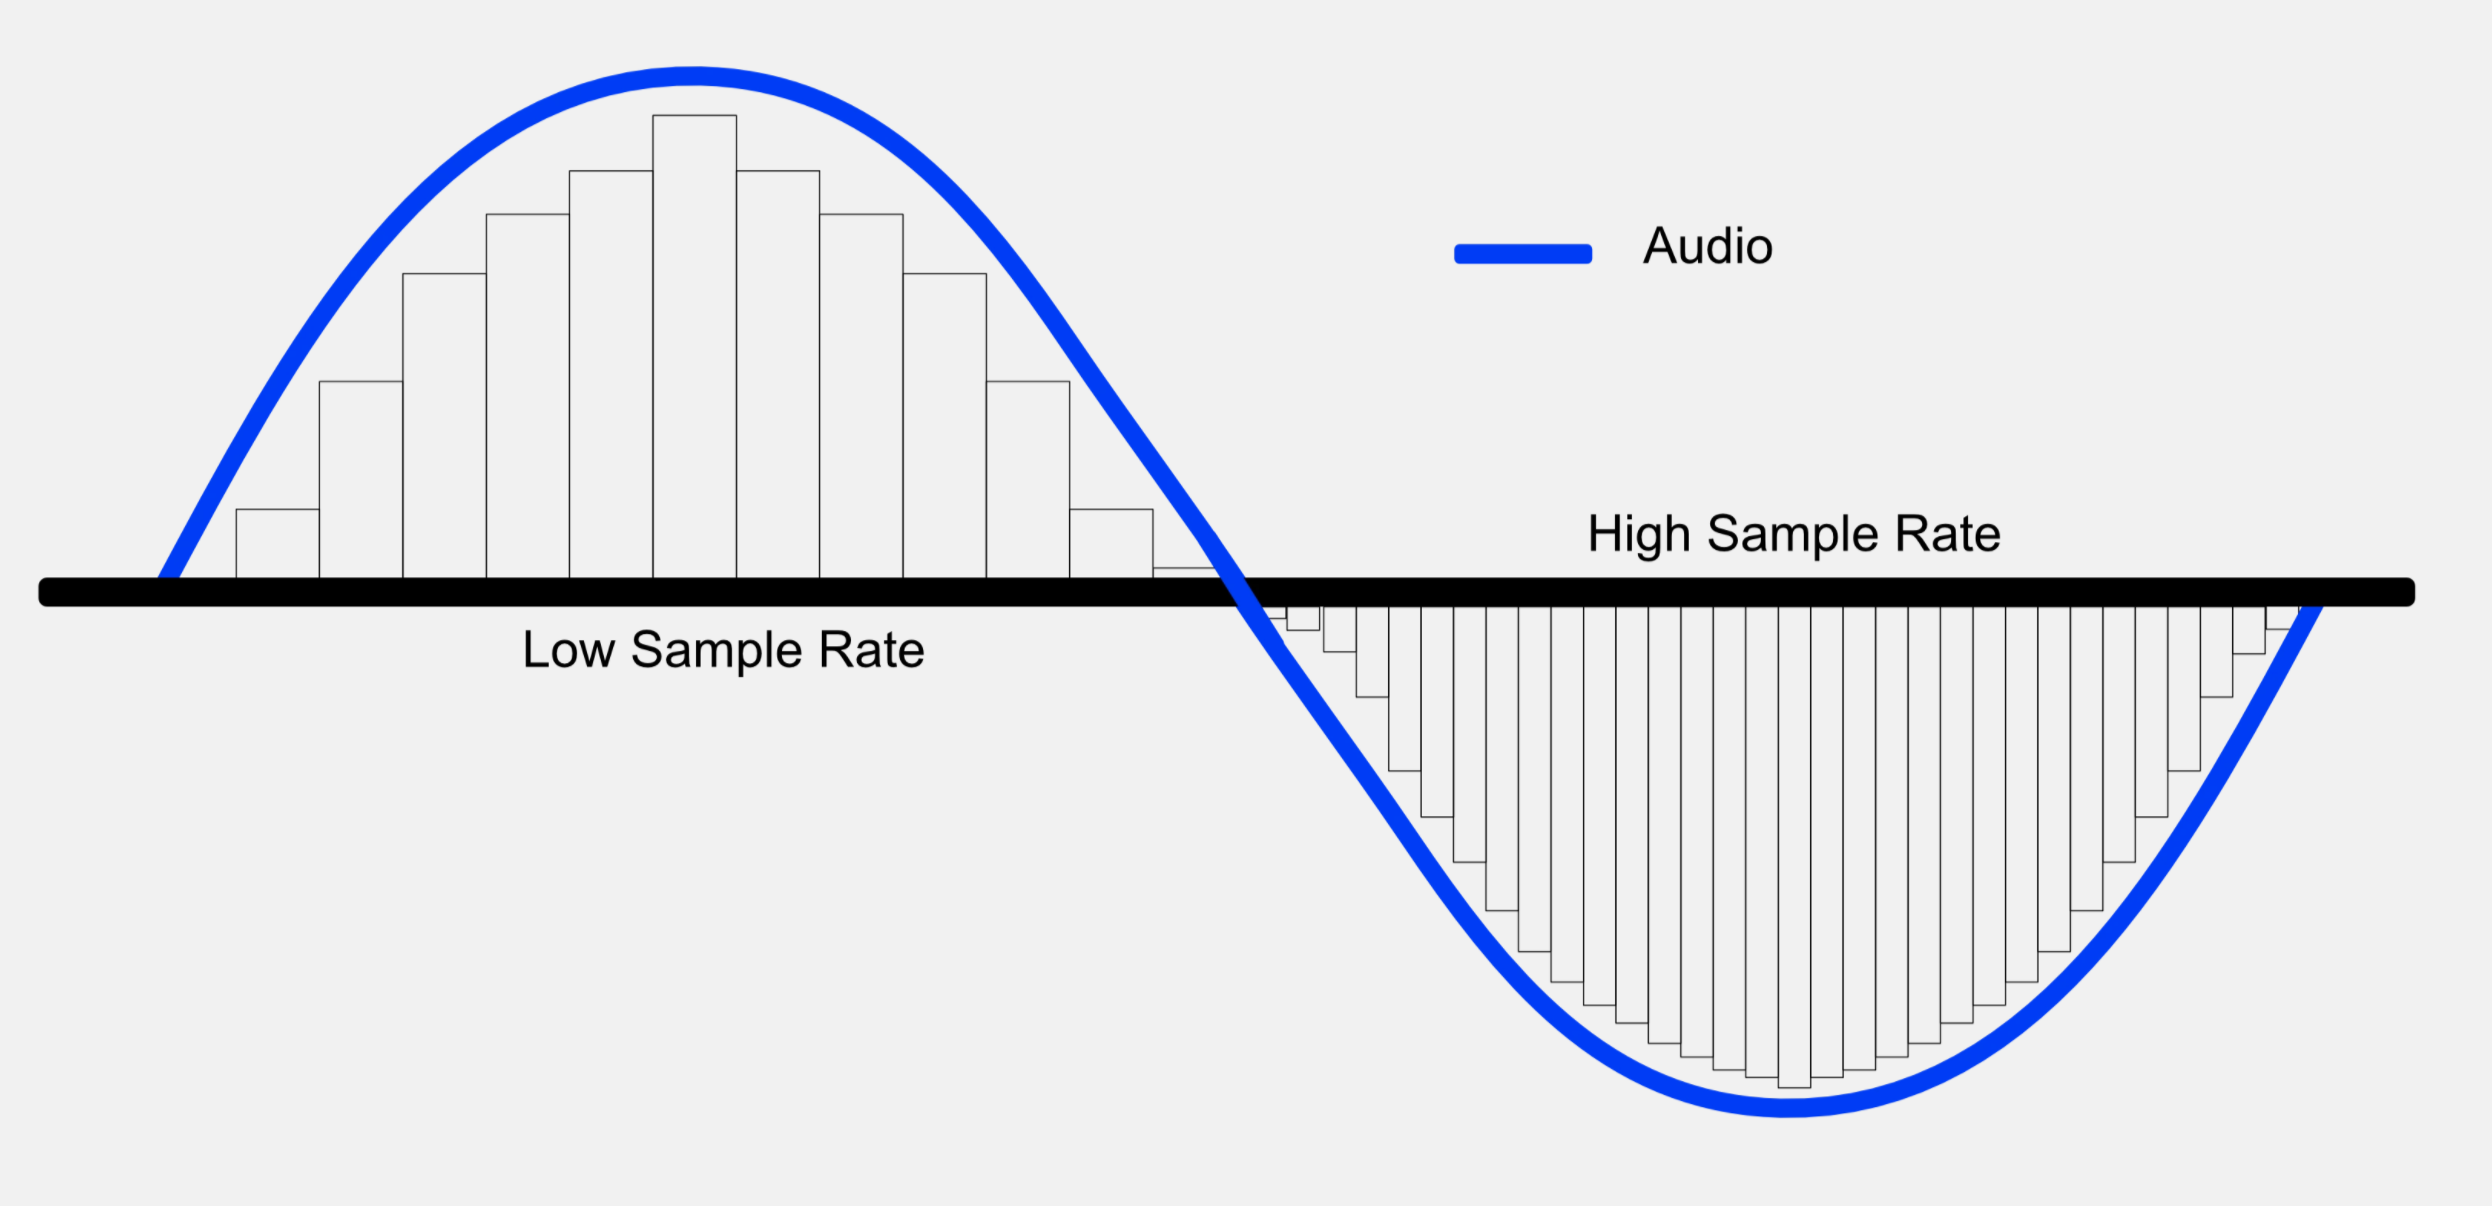
\includegraphics[width=1.0\textwidth]{images/sample-rate.png}
\caption{Примеры различной частота дискретизации (sample rate) для представления аудио}
\label{fig:sample-rate}
\end{figure}

Модели на основе нейронных сетей (NN) для преобразования текста в речь (Text-To-Speech, TTS) превзошли как конкатенативный (concatenative), так и статистический параметрический подходы для синтеза речи с точки зрения качества. Они также значительно упрощают процесс синтеза речи. Традиционно. системы синтеза речи объединяет несколько блоков: модель для извлечения лингвистических признаков из текста, модель длительности, модель предсказания акустических признаков и вокодер на основе обработки сигналов~\cite{taylor}, который служит для преобразования акустических признаков в аудиодорожку. Нейронные TTS системы, как правило, имеют два этапа (Рисунок~\ref{fig:tts-pipeline}). На первом этапе модель генерирует мэл-спектрограммы из текста. На втором этапе вокодер на основе нейронной сети синтезирует речь из мэл-спектрограмм. Большинство моделей TTS на основе NN имеют архитектуру экодер-декодер~\cite{bahdanau} с операциями с механизмом внимания (attention), которая, как было замечено, имеет некоторые общие проблемы:
\begin{enumerate}
    \item A tendency to repeat or skip words~\cite{fastspeech}, due to attention failures when some sub\-sequences are repeated or ignored. To handle this issue, attention-based models use additional mechanisms to encourage monotonic attention \cite{tacotron2,deepvoice3,taigman2017}.
    \item Slow inference relative to parametric models.
    \item No easy way to control prosody nor voice speed, since the length of the generated sequence is automatically determined by the decoder.
\end{enumerate}

\begin{figure}[!ht]
\centering
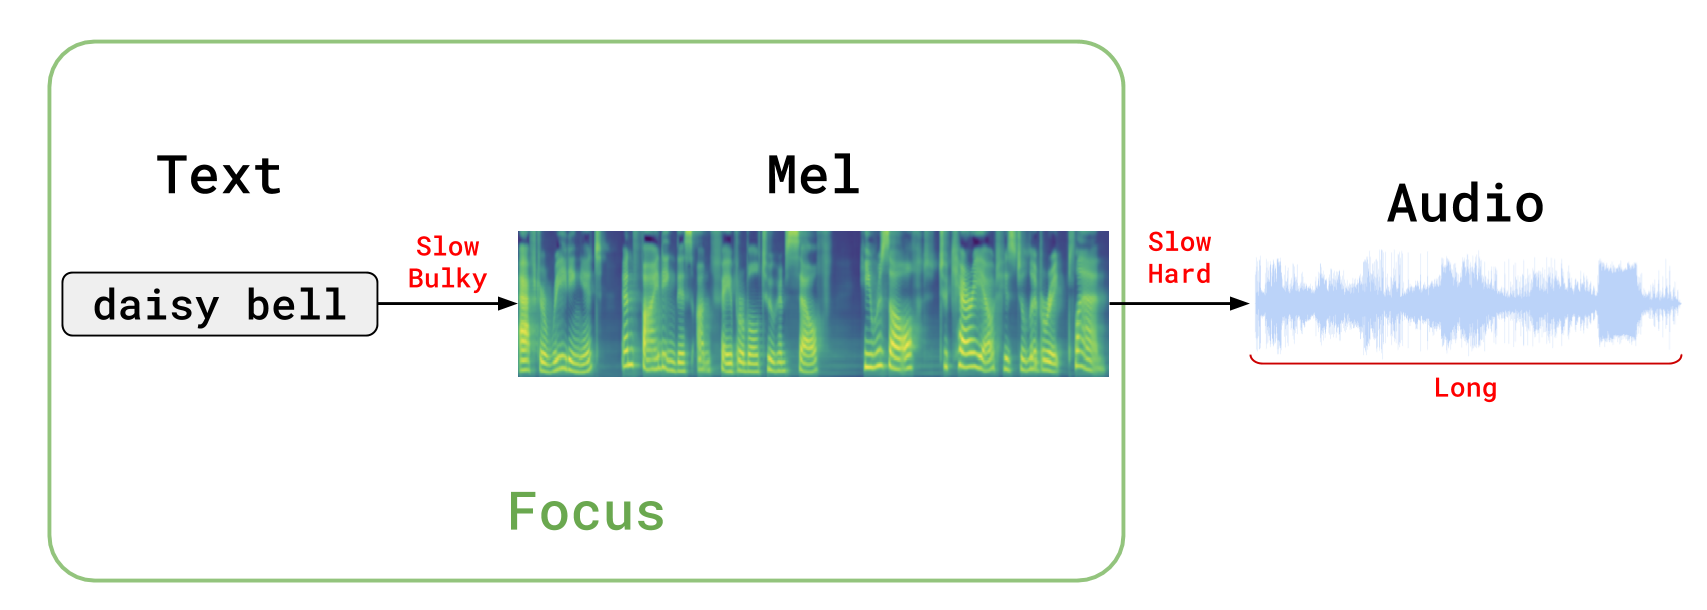
\includegraphics[width=1.0\textwidth]{images/tts-pipeline.png}
\caption{Два шага TTS систем}
\label{fig:tts-pipeline}
\end{figure}

We propose a new neural TTS model to address these three challenges. The model consists of two convolutional networks. The first network predicts grapheme durations. We expand an input text by repeating each symbol according to the predicted duration. The second network generates mel-spectrograms from an expanded text. Finally, we use the WaveGlow~\cite{waveglow} vocoder to synthesize audio from mel-spectrograms (see Figure~\ref{fig:arch}).

To train the grapheme duration predictor, we need the ground truth alignment between input characters and audio. A similar alignment problem exists in automatic speech recog\-nition (ASR) which is addressed by using Connectionist Temporal Classification (CTC). CTC marginalizes over the set of all valid alignments. However, if we take the most likely output at each moment, we can use it for alignment between the input audio and the text output. This alignment is not perfect, and it can have errors. We found that if the ASR model is accurate and has a low character error rate (CER), then we can extract a good-enough alignment between text and audio features. We can use this CTC-based alignment to train the model which will predict grapheme durations for the input text. The explicit grapheme duration predictor replaces attention-based alignment to eliminate word skipping and repeating. Experiments on the LJSpeech dataset show that the speech quality for TalkNet is similar to auto-regressive models.

The convolutional structure of both blocks enables parallel training and inference. This structure enables significantly faster inference, has significantly fewer parameters, and can be trained faster than models with similar quality of generated speech, such as FastSpeech~\cite{fastspeech} and Tacotron 2~\cite{tacotron2}.

\subsection{Обзор методов генерации речи}

A typical statistical parametric TTS pipeline has the following stages: grapheme-to-phoneme conversion, a phoneme duration predictor, an acoustic frame-level feature generator, and a vocoder~\cite{taylor}. Zen et al~\cite{zen-2015,zen-2016} proposed a hybrid NN -- parametric TTS model, where deep neural networks are used to predict the phoneme duration and to generate frame-level acoustic features. The phoneme duration predictor was trained on Hidden Markov Model (HMM)-based phonetic alignments.  

DeepVoice models~\cite{deepvoice1,deepvoice2} also adopt the traditional TTS structure, but they replace all components with NNs. To train the phoneme duration predictor, an auxiliary CTC-based model for phonetic segmentation was used to annotate  data with phoneme boundaries. Tacotron~\cite{tacotron1,tacotron2} is an end-to-end NN which takes characters as input and directly outputs the mel-spectrogram. Tacotron 2 uses an encoder-attention-decoder architecture. The encoder is composed from three convolutional layers plus a single bidirectional LSTM. The decoder is a recurrent neural network (RNN) with location-sensitive monotonic attention.

The sequential nature of RNN-based models limits the training and inference efficiency. There has been a number of TTS models without RNNs. DeepVoice 3~\cite{deepvoice3} replaces an RNN with a fully-convolutional encoder-decoder with monotonic attention. Switching from RNN to a convolutional neural network (CNN) makes training faster, but the model inference is still auto-regressive. Another end-to-end TTS model, which does not use RNNs, is ParaNet~\cite{paranet}. ParaNet is a convolutional encoder-decoder with attention. It distills attention from a teacher auto-regressive TTS model. Lastly, Transformer-TTS~\cite{transformer-tts} replaces an RNN-based encoder-decoder with a Transformer-like  attention-only architecture~\cite{attention-is-all}. Transformer-TTS first converts text to phonemes using a rule-based converter. Using phoneme sequences as input, Transformer-TTS generates mel-spectrograms.  

As with other attention-based models, Tacotron, Transformer-TTS and ParaNet occasionally miss or repeat words~\cite{paranet}. To prevent word skipping and repeating, FastSpeech~\cite{fastspeech} proposes a novel feed-forward Transformer-based model, discarding the conventional encoder-attention-decoder structure. FastSpeech uses an explicit length regulator, which expands the hidden sequence of phonemes according to a predicted duration in order to match the length of a mel-spectrogram sequence. The target phoneme duration is extracted from the attention alignment in an external pre-trained TTS model, Tacotron 2.  % 1
\section{Описание подхода}

TalkNet разбивает генерацию мэл-спектрограммы из текста на два отдельных модуля. Первый модуль, предсказатель длительности, выравнивает входные графемы по времени относительно звуковой дорожки (или мэл-спектрограммы, что то же самое так так длина мэл-спектрограммы линейно зависит от длины аудио). Второй модуль, генератор мэл-спектрограмм, производит генерацию из выровненных по времени входных символов (Рисунок~\ref{fig:arch}). Мы используем конволюционные модели прямого вывода (feed-forward) для обоих модулей, поэтому как обучение, так и вывод не являются авторегрессионными. Это позволяет гораздо быстрее обучаться и делать вывод по сравнению с авторегрессионными моделями. Для обучения предсказателя длительности графем мы извлекли истинностые длительности из выхода CTC предварительно обученной модели разпознавания речи (Automatic-Speech-Recognition, ASR).

\subsection{Извлечение истинных длительностей графем}

Центральная идея TalkNet заключается в использовании модели ASR на основе Connectionist Temporal Classification (CTC) функции ошибки для извлечения выравниваний графем. CTC присваивает вероятность каждому из символов алфавита и использует вспомогательный пустой символ $\sim$. Первым шагом мы схлопываем соседние повторяюшиеся символы в выводе, подсчитывая таким образом длительность каждого символа. Пустой символ выступает как промежуточное состояние между двумя соседними графемами, и его длительность соответствует длительности перехода от одного символа к другому. Для каждого временного шага мы выбираем наиболее вероятный символ из выходных данных CTC (Рисунок~\ref{fig:ctc}).

\begin{figure}[!ht]
\centering
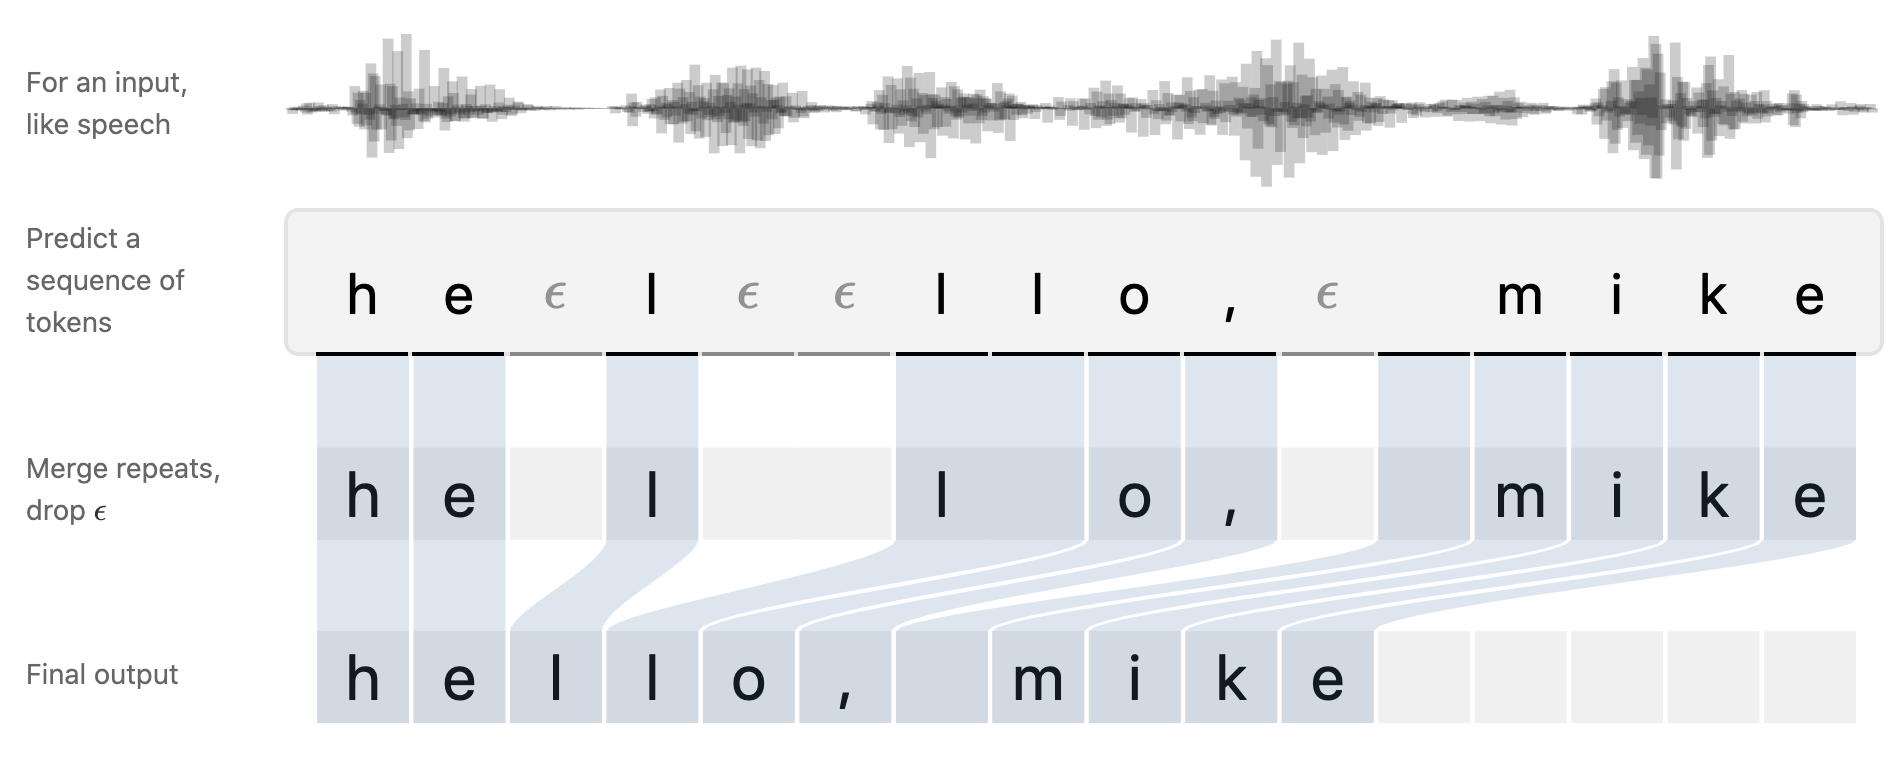
\includegraphics[width=1.0\textwidth]{images/snippets/ctc.png}
\caption{Пример работы CTC алгоритма~\cite{hannun2017sequence}. Соседние буквы схлопываются, а $\epsilon$ ($\sim$ в нашей нотации) служит разделительным вспомогательным символом.}
\label{fig:ctc}
\end{figure}

CTC -- это функция ошибки, используемая для этапа обучения. Поэтому, выход CTC часто бывает неточен. Однако, задача ASR решена намного лучше TTS, поэтому ошибка все еще меньше. Мы выравниваем выход CTC с истинным отрывком текста для того чтобы максимально устранить влияние ошибки. Мы используем функцию \textit{pairwise2} из пакета Biopython~\cite{biopython}, которая выравниваем два строковых представления побуквенно, используя наименьшее количество операции добавления и удаления символов. Затем мы удаляем все неправильные символы в выводе CTC, добавля их длительность к ближайшему пустому, а также добавляем недостающие символы и устанавливаем их длительность в $0$. Затем для всех символов с предсказанной длительностью 0 мы устанавливаем длительность в 1, вычитая 1 из почти самого большого соседнего $\sim$, чтобы сумма всех длительностей графемы была равна длине мэл-спектрограммы (Рисунок~\ref{fig:alignment}).

\begin{figure}[!ht]
\centering
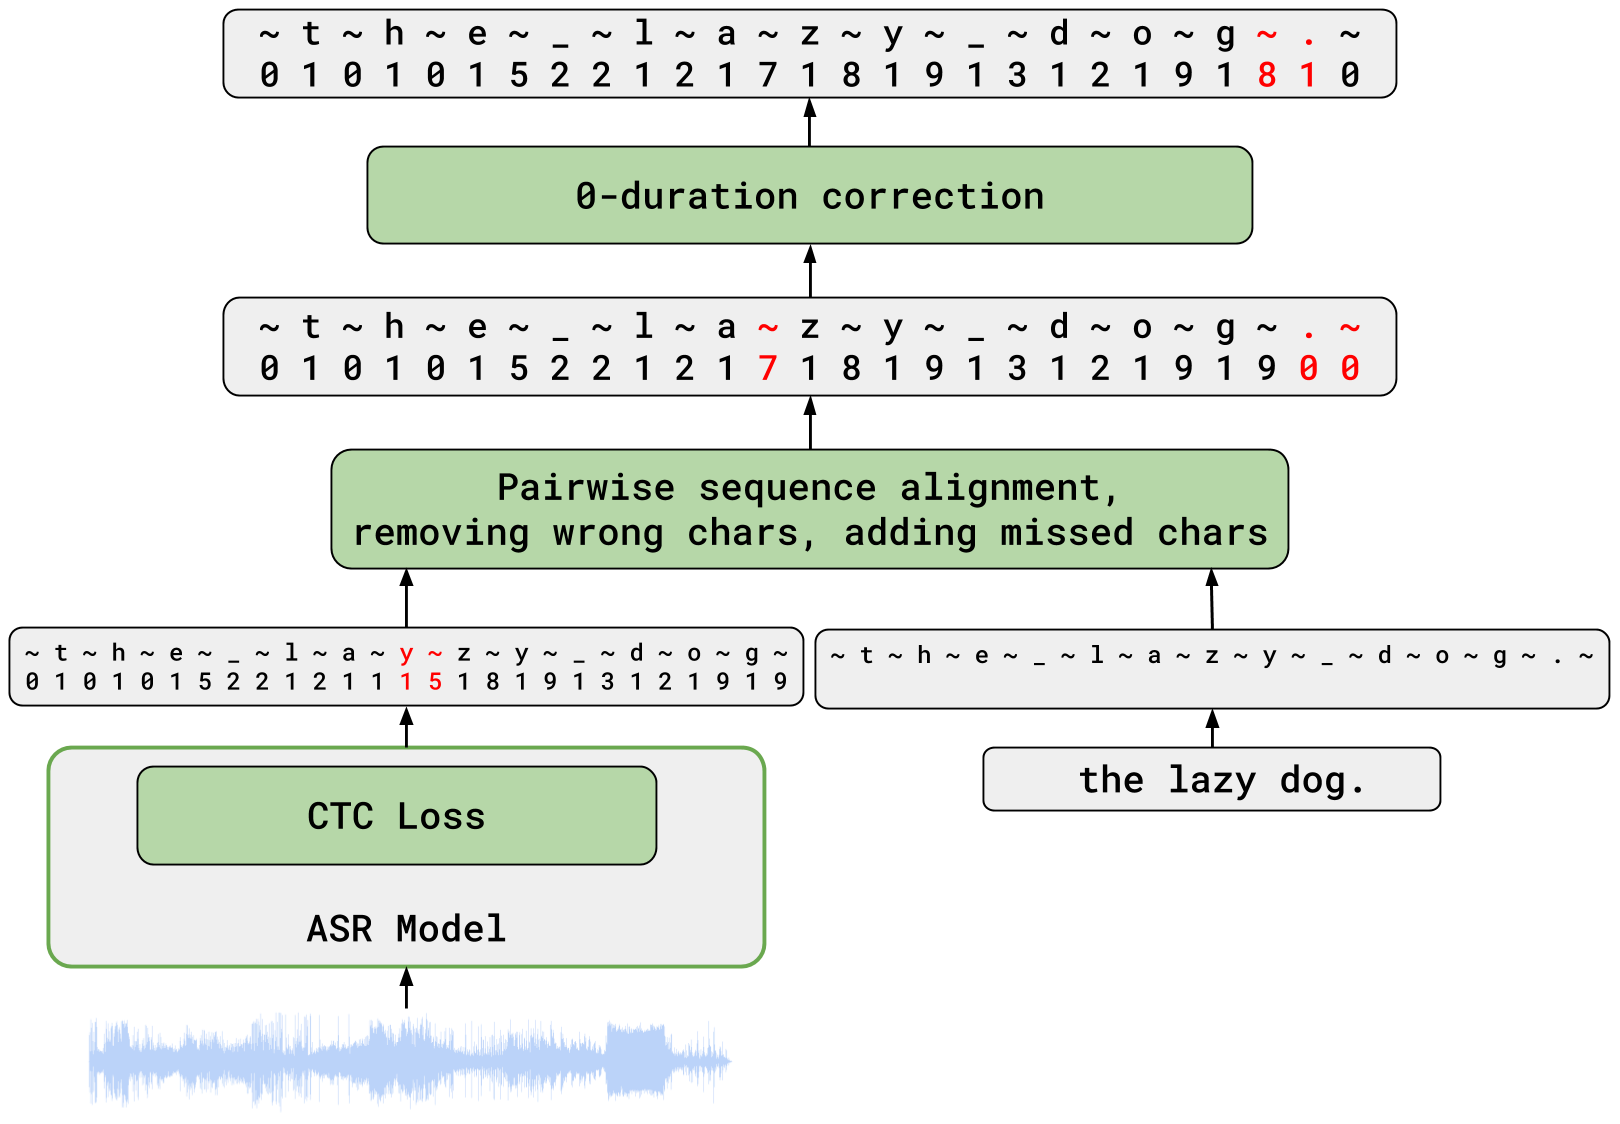
\includegraphics[width=1.0\textwidth]{images/alignment.png}
\caption{Извлечение длительности графемы из вывода CTC. Мы используем $\sim$ для обозначения пустого символа.}
\label{fig:alignment}
\end{figure}

В качестве модели с CTC выводом для задачи разпознования текста (ASR) мы используем QuartzNet~\cite{quartznet}. QuartzNet (Рисунок~\ref{fig:qn}) -- это полностью-коволюционная нейронная архитектура, основными достоинствами которой являются:
\begin{itemize}
    \item Низкое количество параметров (около 18 миллионов), которое было достигнуто за счет использования depthwise separable~\cite{kaiser2017depthwise} конволюций, являющихся математическим приближение обычных конволюций.
    \item Простая неавторегрессионная архитектура с базовыми операциями из глубокого обучения (конволюции, нелинейности, батч-нормализация и дропаут), позволяющяя ускорить процесс обучения и вывода (inference).
    \item CTC функция в качестве функции ошибки в декодере, которая не содержит допольнительных параметров и обеспечивает быстрый вывод.
\end{itemize}

\begin{figure}[!ht]
\centering
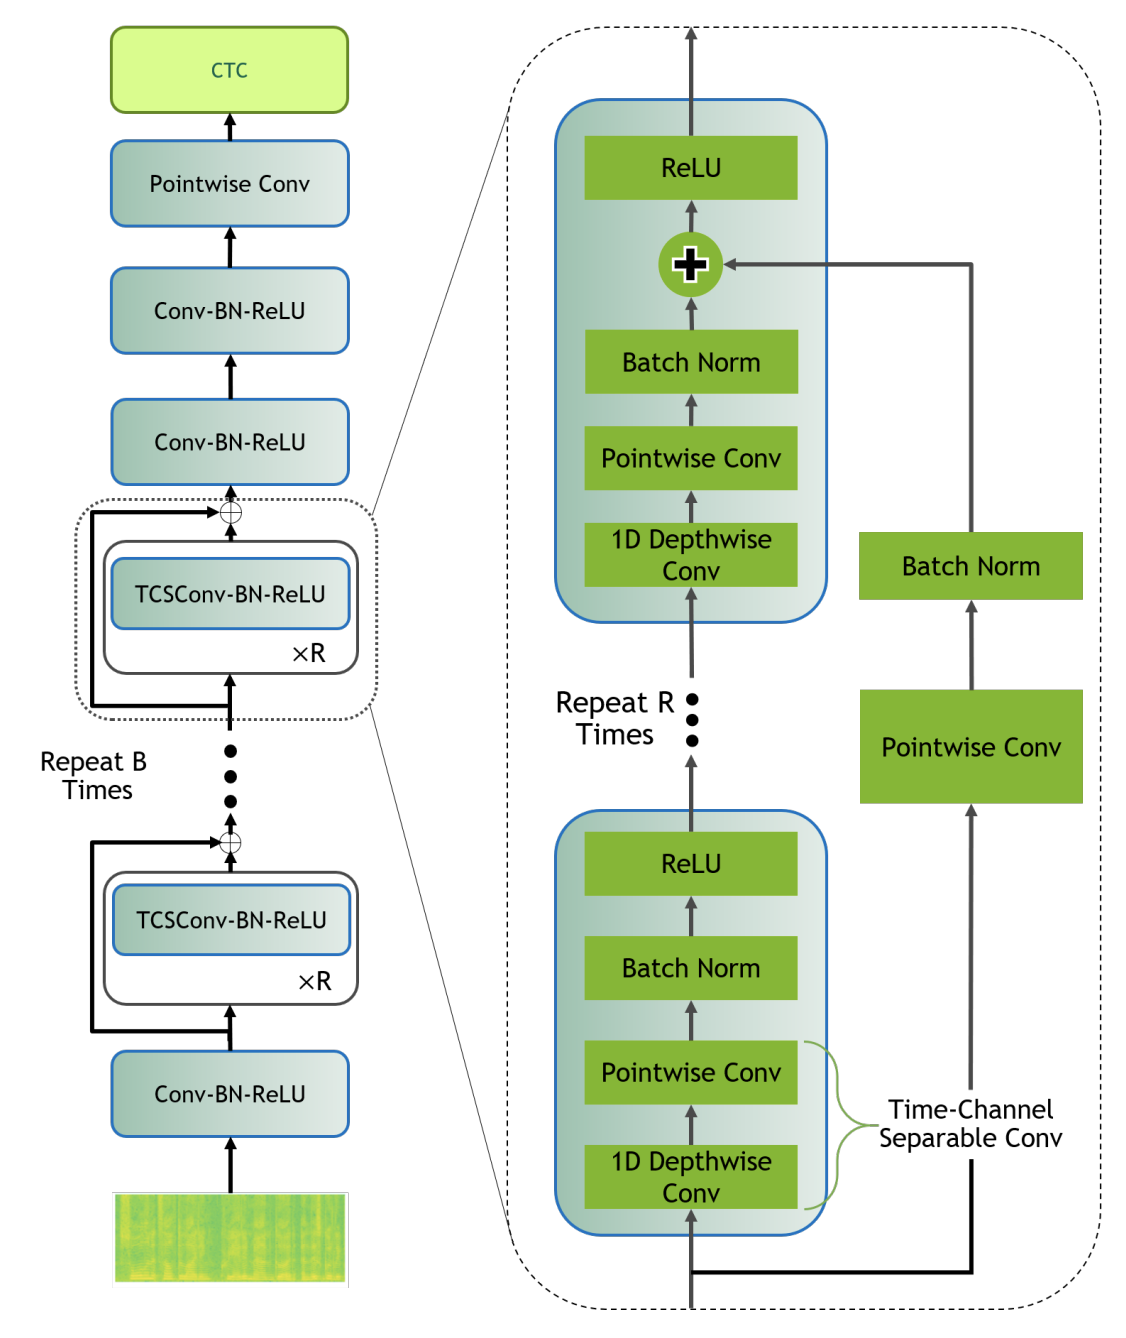
\includegraphics[width=1.0\textwidth]{images/qn.png}
\caption{Архитектура QuartzNet 15x5}
\label{fig:qn}
\end{figure}

Для получения истинных длительностей графем мы используем QuartzNet 15x5 (15 блоков по 5 повторений). Выход такой модели по длине в 2 раза меньше входной мэл-спектрограммы. Причина -- в самой первой конволюции выставлен параметр $\texttt{stride}=2$ (Рисунок~\ref{fig:stride-2}). QuartzNet использует удвоение шага в самом начале, так как для любого примера длина выходного текста как минимум в два раза меньше длины мэл-спектрограммы, поэтому такой трюк позволяет сократить количество вычислений вдвое. Однако, это так же уменьшает длительность каждого символа в выходе CTC. Чтобы сравнять сумму длительностей с длиной мэла, мы модифицируем QuartzNet, устанавливая $\texttt{stride}=1$ для первого слоя. Заметим так же что это не убирает возможность воспользоваться предобученной моделью, загрузив веса перед обучением для дообучения (fine-tuning) -- размеры, форма и количество ядер (kernels) конволюций остается неизменным. Соотвестсвенно, не изменяются и размеры матриц и векторов с весами.

\begin{figure}[!ht]
\centering
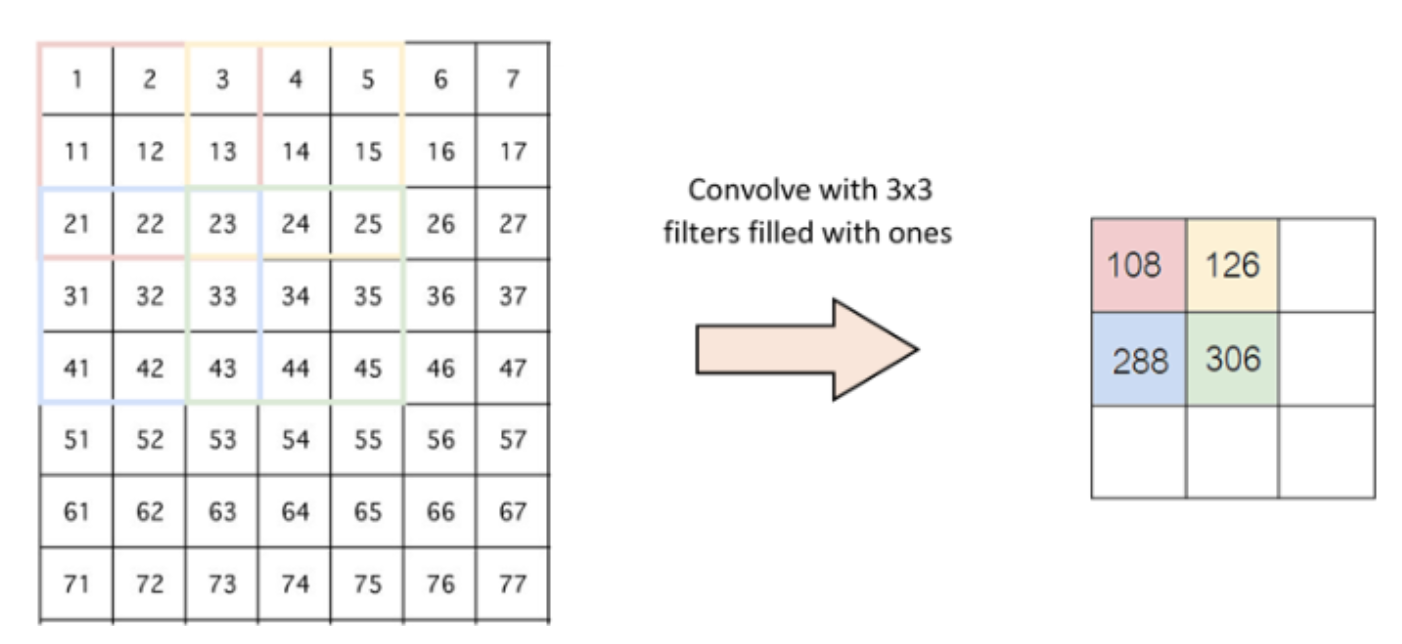
\includegraphics[width=1.0\textwidth]{images/snippets/stride-2.png}
\caption{Пример работы конволюций с удвоенным шагом}
\label{fig:stride-2}
\end{figure}

Мы дообучаем QuartzNet 15x5 на данных из датасета LibriTTS~\cite{libritts}. LibriTTS это набор данных из того же источника, что и LibriSpeech, на котором успешно обучался оригинальный QuartzNet. Однако, LibriTTS использует другую обработка данных, которая более подходит для задач генерации речи, нежели разпознования речи. В частности, LibriTTS обрезает отрывки аудио по большим паузам, оставляет всю пунктуацию нетронутой (для экспрессивности речи), а также разворачиваем некоторые числа и буквенные сокращения. Для токенизации входного текста (разбиения на символы) мы также оставляем всю пунктуацию, давая возможность CTC самому назначит длительность каждому сивмолу. При дообучении QuartzNet на LibriTTS мы достигаем побуквенной ошибки (Char-Error-Rate, CER) порядка $4.51\%$ на части dev-clean и порядка $3.54\%$ на тестовой части LJSpeech~\cite{ljspeech}. Выравнивание, полученное из CTC, используется для обучения предиктора длительности графемы.

Таким образом, вместо того чтобы использовать другую преодобученную TTS модель в качестве учителя для получения длительностей графем, как это делалось в модели FastSpeech~\cite{fastspeech}, мы представляем метод в котором используется ASR модель. Ошибка, получаемая в CTC гораздно меньше ошибки при генерации речи, поэтому такой способ позволяет снять жесткое ограничение на качество, задаваемой моделью учителя.

\subsection{Grapheme duration predictor}

This model predicts the length of the mel-spectrogram part corresponding to each gra\-pheme in the input including punctuation. First, the grapheme duration predictor inserts a blank symbol $\sim$ between every two input characters. Next, it predicts the duration for each input character. We expand the sequence of input characters by repeating each character according to the predicted duration  (Figure~\ref{fig:durs}).

\begin{figure}[!ht]
\centering
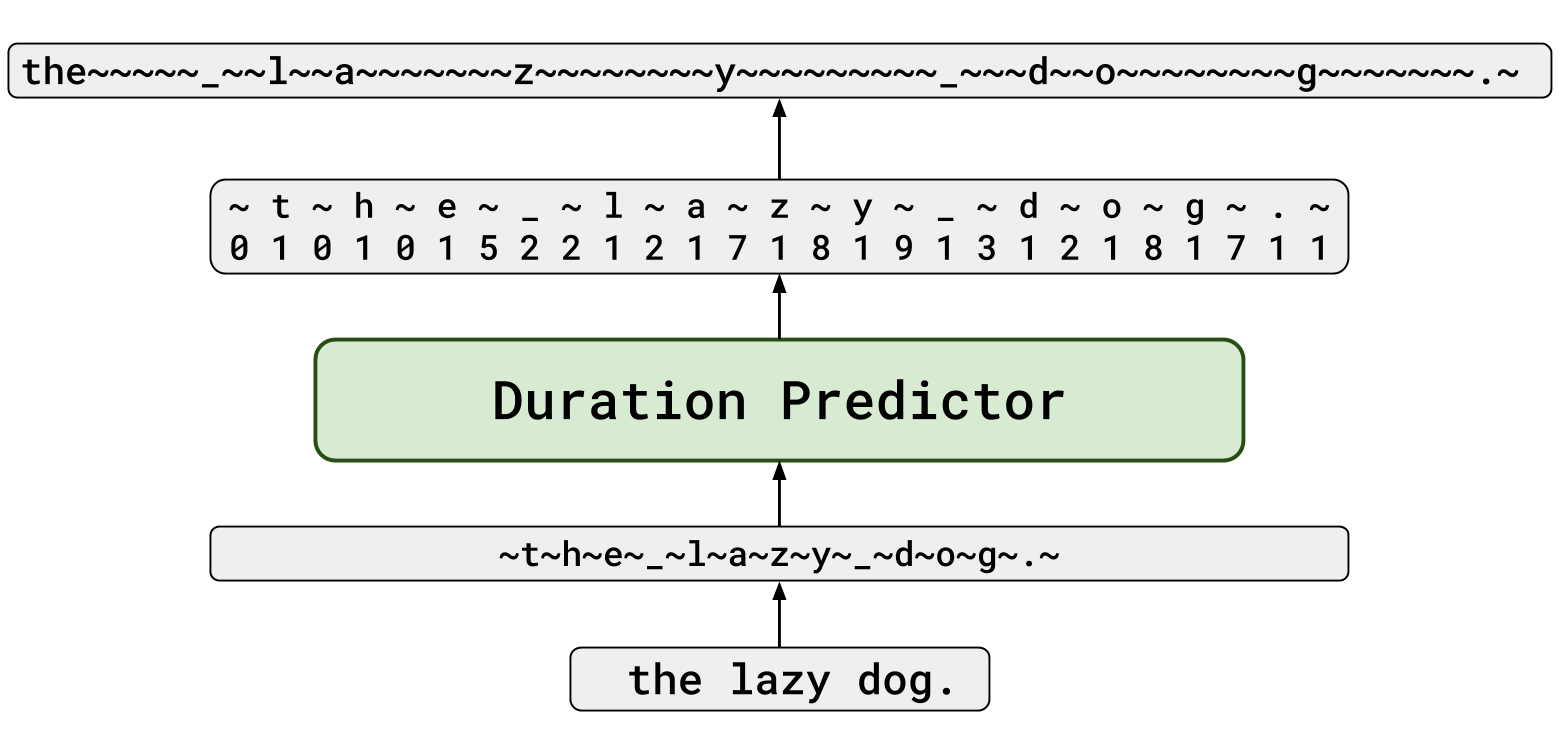
\includegraphics[width=1.0\linewidth]{images/durs.png}
\caption{Grapheme duration prediction.}
\label{fig:durs}
\end{figure}

The grapheme duration predictor model is a 1D time channel separable convolutional NN based on QuartzNet architecture~\cite{quartznet}. The model has $5$ residual blocks with 5 sub-blocks per block. A sub-block consists of a 1D time-channel separable convolution, a 1x1 pointwise convolutions, batch norm, ReLU, and dropout (see Figure~\ref{fig:qn-block}). There are two additional layers: the grapheme embedding layer, and a $1x1$ convolutional layer before loss function (see Table~\ref{tab:durs-model}).

\begin{figure}[!ht]
\centering
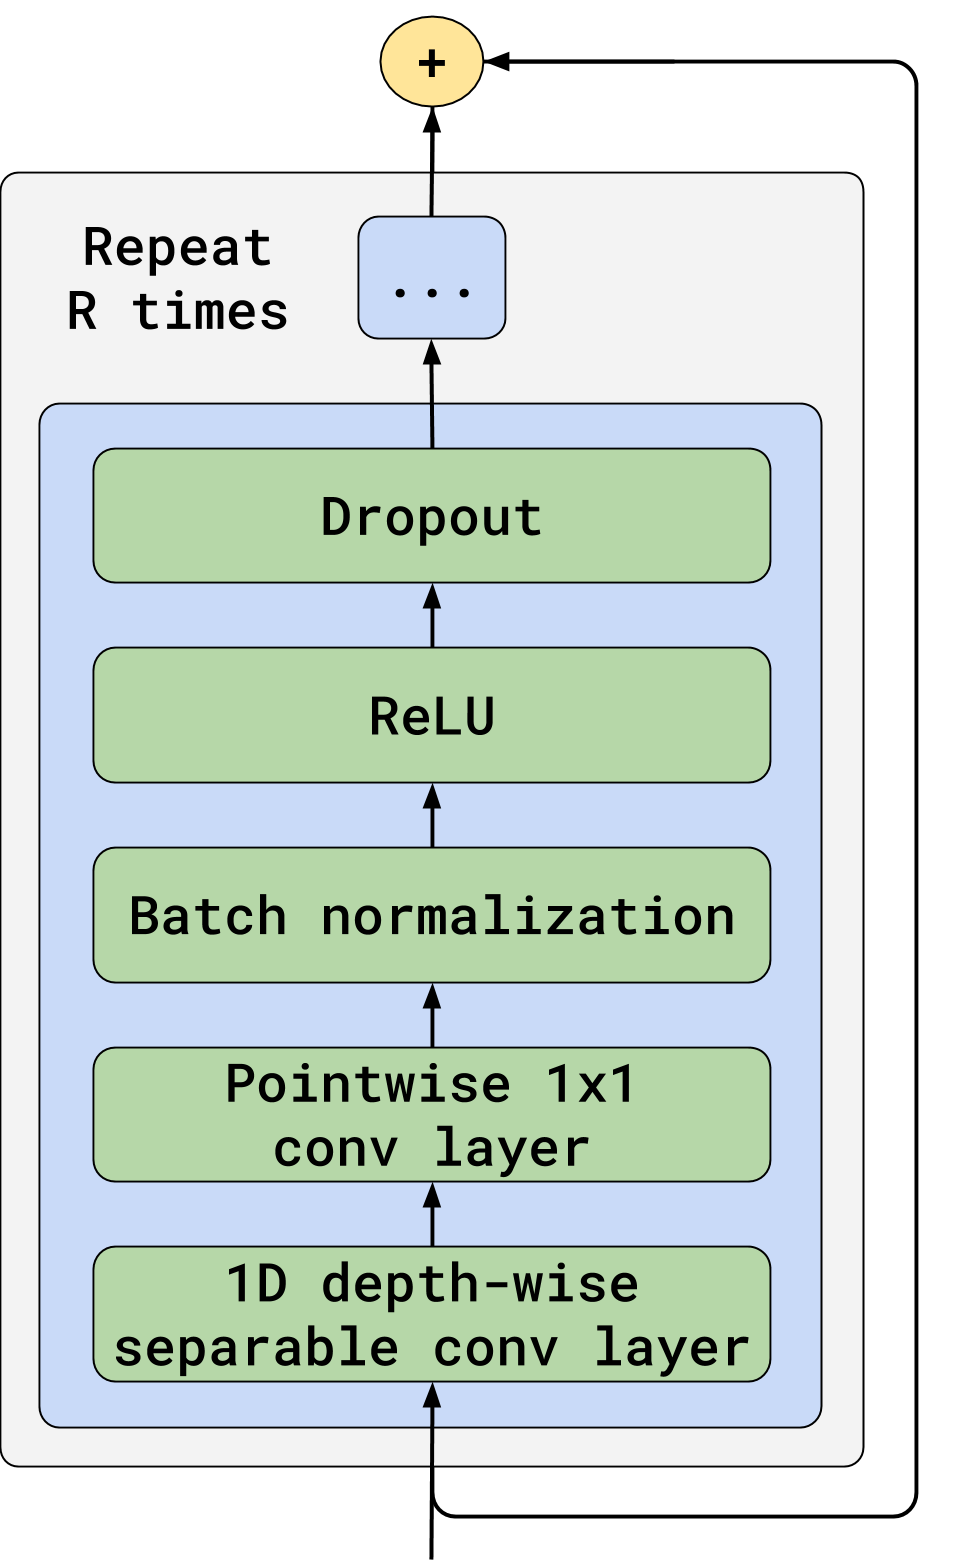
\includegraphics[width=0.8\linewidth]{images/qn-block.png}
\caption{Basic QuartzNet block. Both grapheme duration predictor and mel-spectrogram generator are 1D time-channel convolutional networks based on QuartzNet~\cite{quartznet}.}
\label{fig:qn-block}
\end{figure}

We train a duration predictor using $L_2$ loss with logarithmic targets, similar to~\cite{fastspeech}. We also tried cross-entropy (XE) loss with each class corresponding to the character duration. We used a log scale for large durations since grapheme duration distribution has a long tail (Figure~\ref{fig:durs-dist}). Cross entropy has slightly higher accuracy (see Table~\ref{tab:durs-results}). We choose $L2$ since a speech generated with L2 loss got slightly higher mean-opinion-score (MOS) in our evaluation studies.

\begin{figure}[!ht]
\centering
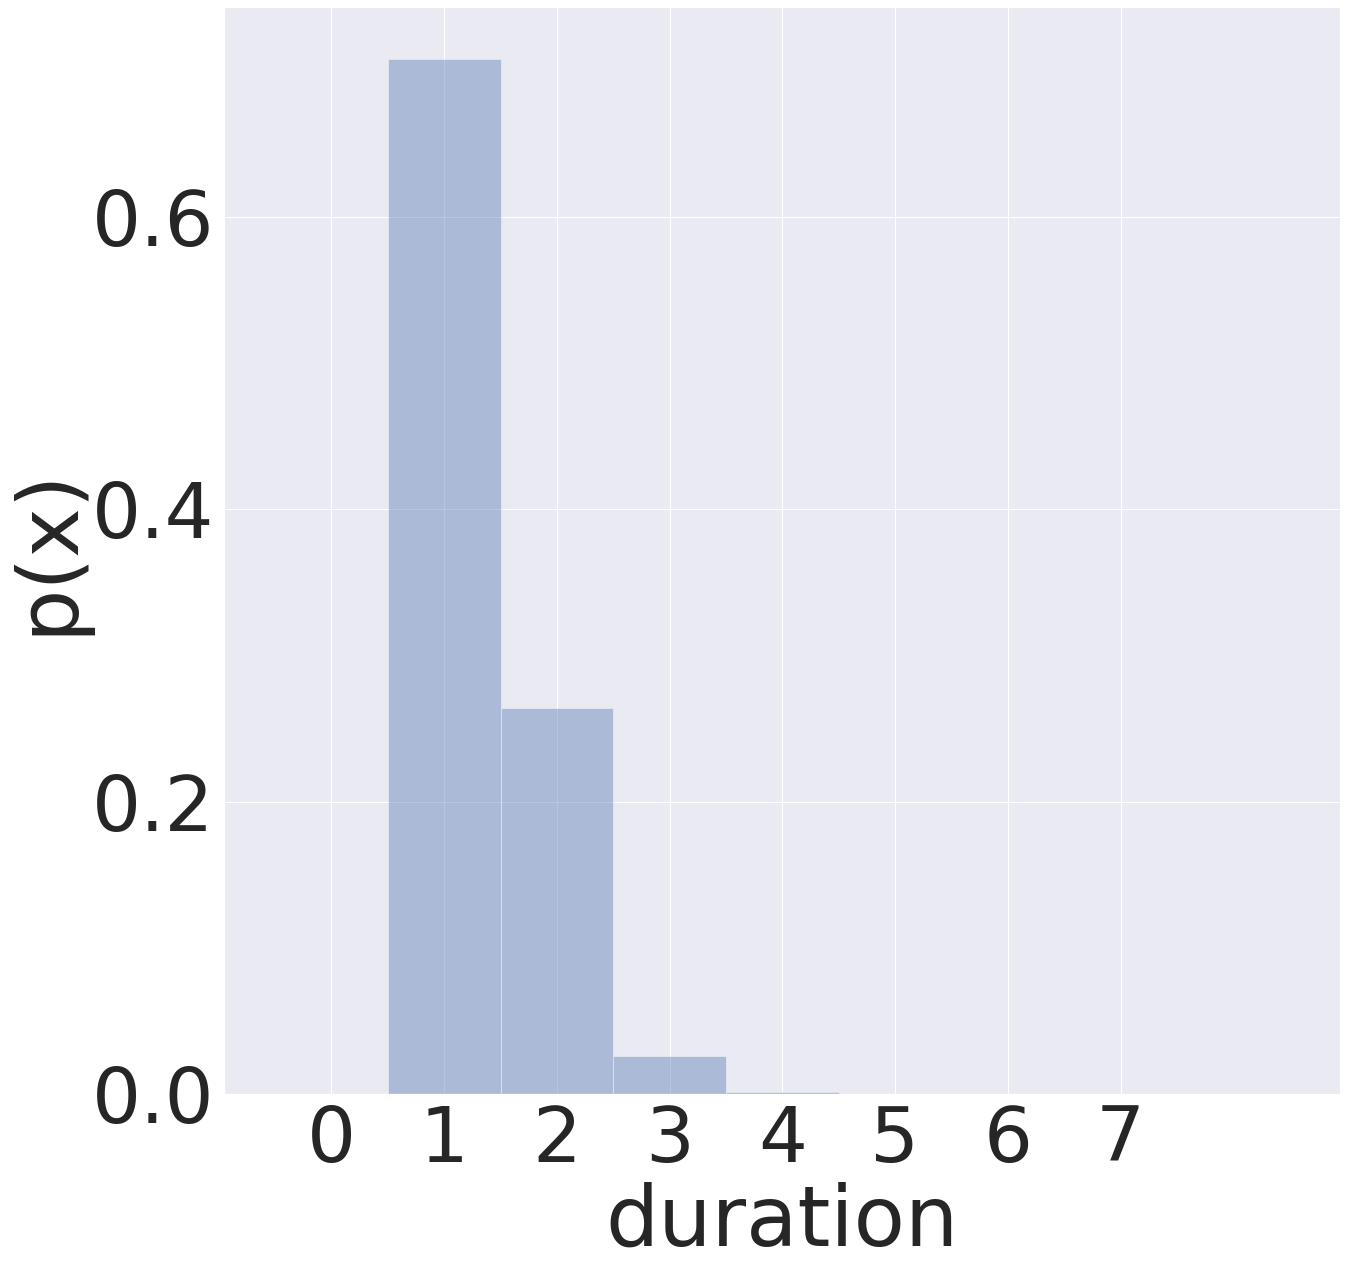
\includegraphics[width=.48\linewidth]{images/durs-dist.png}
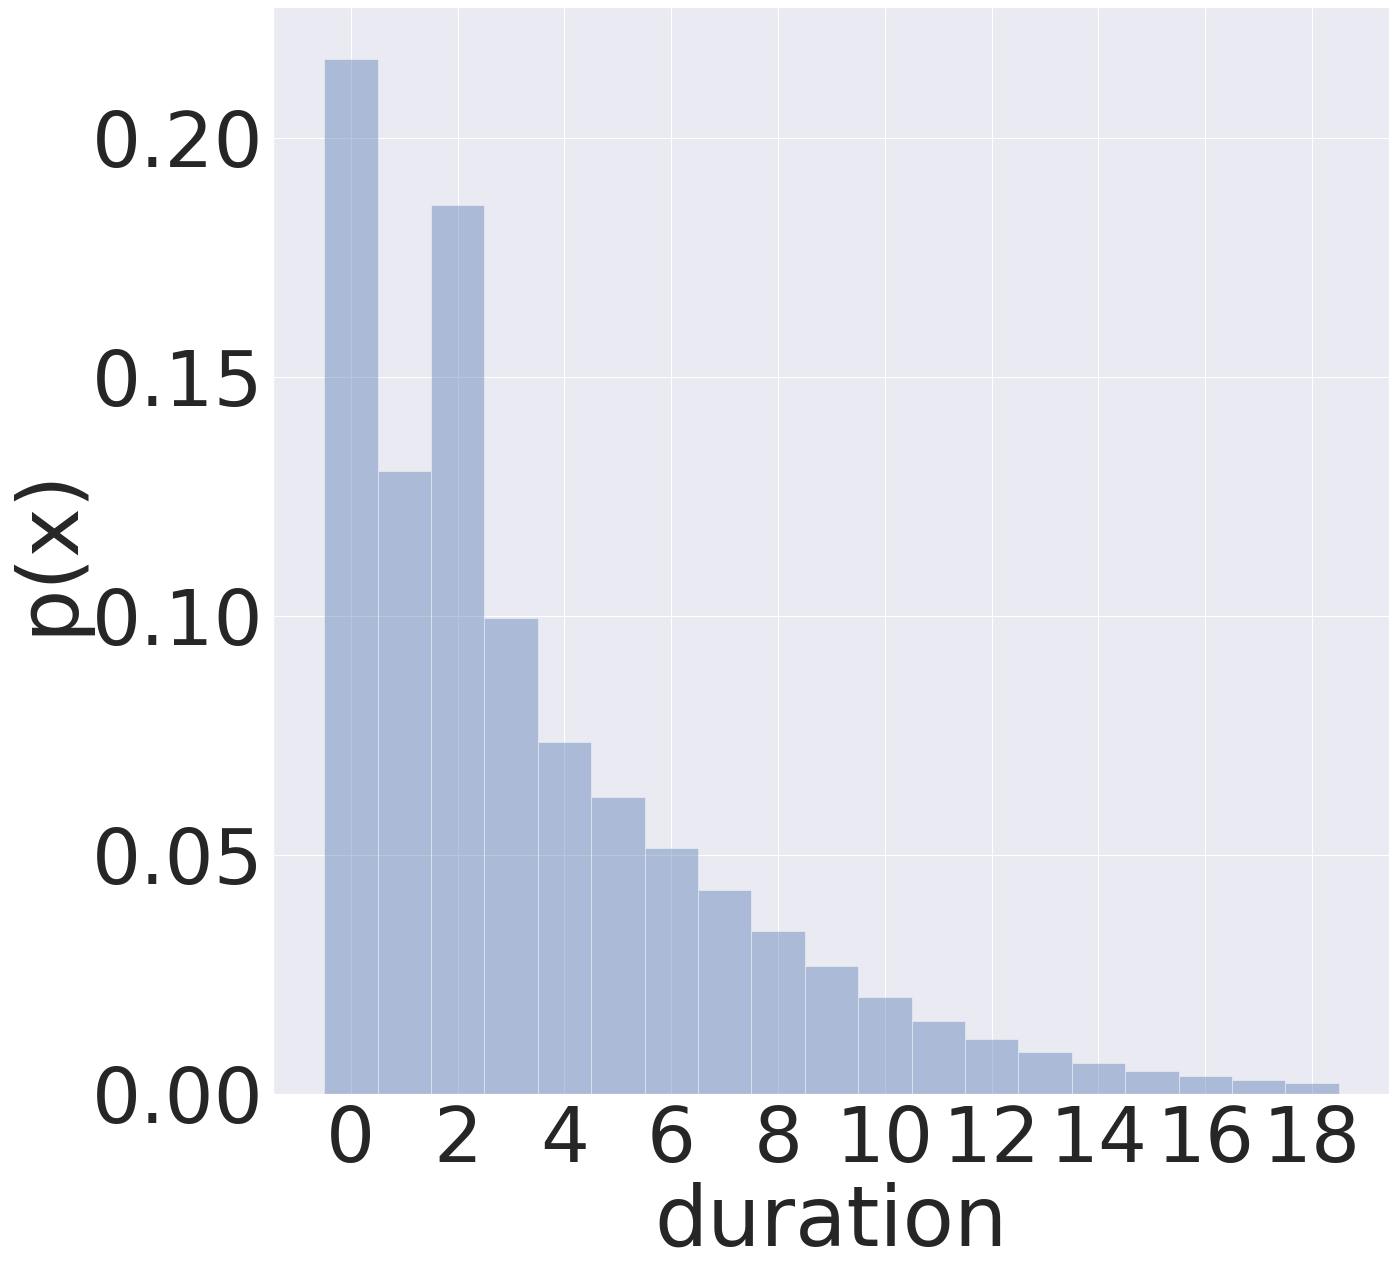
\includegraphics[width=.48\linewidth]{images/blanks-dist.png}
\caption{The duration's distribution for characters (left) and for blanks (right) based on CTC output for LJSpeech dataset. The maximum duration for characters is $7$, and for blanks -- $493$.}
\label{fig:durs-dist}
\end{figure}

\begin{table}[!ht]
\centering
\scalebox{1.0}{
\begin{tabular}{c c c c c} 
\toprule
\textbf{Block} &
\textbf{\thead{\# Sub\\Blocks}} &
\textbf{\thead{\# Output\\Channels}} &
\textbf{Kernel Size} &
\textbf{Dropout} \\
\midrule
Embed & 1 & 64  & 1 & 0.0  \\
Conv1 & 3 & 256 & 3 & 0.1  \\
$B_1$ & 5 & 256 & 5 & 0.1  \\
$B_2$ & 5 & 256 & 7 & 0.1  \\
$B_3$ & 5 & 256 & 9 & 0.1  \\
$B_4$ & 5 & 256 & 11 & 0.1 \\
$B_5$ & 5 & 256 & 13 & 0.1 \\
Conv2 & 1 & 512 & 1 & 0.1  \\
Conv3 & 1 & $32$ & 1 & 0.0 \\
\midrule
\textbf{Params, M} & & & & \textbf{2.3} \\
\bottomrule
\end{tabular}
}
\caption{Grapheme duration predictor is based on QuartzNet 5x5.}
\label{tab:durs-model}
\end{table}

\begin{table}[!ht]
\centering
\scalebox{1.0}{
\begin{tabular}{c c c c c c c} 
\toprule
\textbf{Method} &
\textbf{MSE} &
\textbf{Accuracy, $\%$} &
$\mathbf{|P - T| \leq 1}$ &
$\mathbf{|P - T| \leq 3}$\\
\midrule
$L_2$ & 7.81 & 67.69 & 91.90 & 97.17 \\
XE & 10.46 & 69.42 & 92.90 & 97.40 \\
\bottomrule
\end{tabular}
}
\caption{Duration's predictor results, LJSpeech test set. $P$ -- predicted, $T$ -- target.}
\label{tab:durs-results}
\end{table}

\subsection{Mel-spectrogram generator}

The second module generates mel-spectrogram from the expanded text. The mel-spectro\-gram generator is a 1D convolutional network based on the same QuartzNet architecture. It has $9$ blocks with 5 sub-blocks (see Table~\ref{tab:mels-model}). The mel-spectrogram generator was trained with a mean square error (MSE) loss.

Instead of allocating a separate embedding for blank symbol, we use a linear combination of embeddings for the neighboring graphemes. Namely, if the blank symbol $\sim$ is located between the  characters $a$ and $b$ and the blank duration is $d$, then the embedding $E$ for the blank symbol located at the distance $t$ from $a$ would be $E(\sim, t) = \dfrac{d+1-t}{d+1} \cdot E(a) + \dfrac{t}{d+1} \cdot E(b)$.

\begin{table}[!ht]
\centering
\scalebox{0.85}{
\begin{tabular}{c c c c c} 
 \toprule
  \textbf{Block} &
  \textbf{\thead{\# Sub\\Blocks}} &
  \textbf{\thead{\# Output\\Channels}} &
  \textbf{Kernel Size} &
  \textbf{Dropout} \\
 \midrule
Embed & 1 & 256 & 1 & 0.0 \\
Conv1 & 3 & 256 & 3 & 0.0 \\
$B_1$ & 5 & 256 & 5 & 0.0 \\
$B_2$ & 5 & 256 & 7 & 0.0 \\
$B_3$ & 5 & 256 & 9 & 0.0 \\
$B_4$ & 5 & 256 & 13 & 0.0 \\
$B_5$ & 5 & 256 & 15 & 0.0 \\
$B_6$ & 5 & 256 & 17 & 0.0 \\
$B_7$ & 5 & 512 & 21 & 0.0 \\
$B_8$ & 5 & 512 & 23 & 0.0 \\
$B_9$ & 5 & 512 & 25 & 0.0 \\
Conv2 & 1 & 1024 & 1 & 0.0 \\
Conv3 & 1 & 80 & 1 & 0.0 \\
\midrule
\textbf{Params, M} & & & & \textbf{8.5} \\
\bottomrule
\end{tabular}
}
\caption{Mel-spectrogram generator is based on QuartzNet~9x5.}
\label{tab:mels-model}
\end{table}  % 2
\section{Решение}

\subsection{Данные для обучения}

Стандартной практикой в области генерации данных является разделение датасетов на одноголосные (single-speaker) и многоголосные (multi-speaker), количество спикеров у которых доходит до нескольких тысяч, а количество минут чистой речи на каждого спикера -- около $20$~\cite{libritts}. Предварительные эскперименты с TalkNet показали, что для обучения эффективной многоголосной системы потребуется дополнительная контекстная информация о характере голоса, без которой сложно уловить зависимости между аудио и получить хорошее качество звучания. К примеру, в качестве эмбеддинга спикера можно использовать Global Style Token~\cite{wang2018style} или похожие эксперименты. Multi-Speaker TalkNet оставлено авторами как одно из направлений для будущей работы.

В рамках данной работы мы решили использовать данные из датасета LJSpeech~\cite{ljspeech}, который является стандартом де-факто для тестирования процесса генерации и позволяет легко сравнивать результаты с другими подходами. LJSpeech это одноголосый набор данных из 13100 отрывков семи аудиокниг документального жанра на английском языке. Размер отрывков варьируется от 1 до 10 секунд. Каждому отрывку в соответствие поставлена текстовая транскрипция с сохранением пунктуации и нормализацией чисел, денежных знаков и некоторых сокращение. Суммарная протяженность аудио -- около 24 часов.

Мы произвольно разделили набор данных на три части: $12,500$ для обучения, 300 для валидации и 300 для тестирования. Для обработки текста была использована стандартная токенизация с понижением регистра и использованием пунктуации. Таким образом мы полностью сохраняем эспрессивность текста и помогаем модели правильным образом выучить паузы, повышение тона, выделение голосом частей текста и другие особенности речи.

Как было уже сказано выше, мы не предсказывает "сырую" аудио дорожку напрямую, а используем промежуточное представление в виде мэл-спектрограмм. Такое компактное представление строится конструктивно и детерменированно из аудио с помощью оконного преобразования Фурье. Суть этой операции в последовательном применении преобразования Фурье к коротким кусочкам речевого сигнала, домноженным на некоторую оконную функцию. Результат применения оконного преобразования —- это матрица, где каждый столбец является спектром короткого участка исходного сигнала (Фигура~\ref{fig:mel-example}).

\begin{figure}[!ht]
\centering
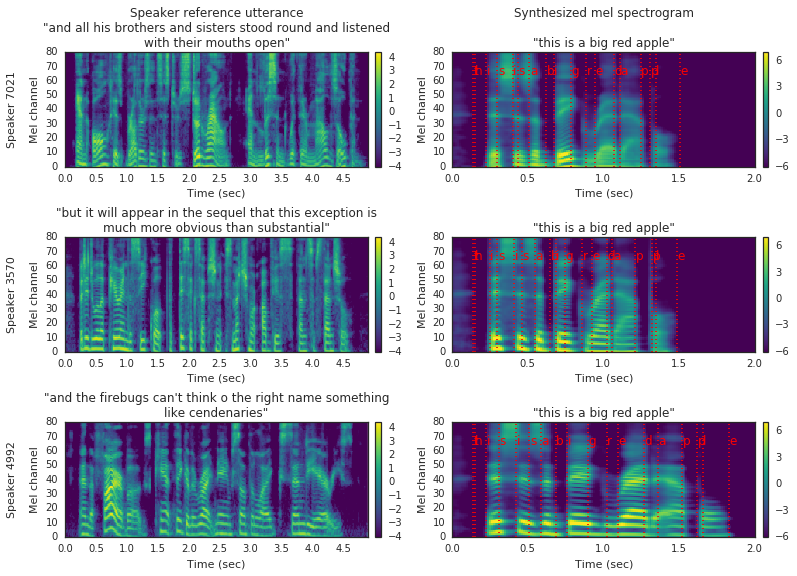
\includegraphics[width=1.0\textwidth]{images/mel-example.png}
\caption{Примеры полученных мэл-спектрограмм с выровненным текстом}
\label{fig:mel-example}
\end{figure}

Для построения мэлов мы использование библиотеку \texttt{librosa}. Мы преобразуем аудиосигналы в мэл-спектрограммы с помощью кратковременного преобразования Фурье (Short-Time Fourier Transform, STFT), используя размер окна в 50 мс с шагом в 12.5 мс, окно вида "hann" и логарифмируем результат. Более подробные характеристики преобразования: $\texttt{win\_length}=1024, \texttt{hop\_length}=256, \texttt{n\_fft}=1024, \texttt{low\_freq}=0$ и $\texttt{high\_freq}=80$.

\subsection{Обучение предсказателя длительности графем}

Как уже было сказано выше, часть TalkNet'а ответственная за предсказание длительности графен обучается отдельно. На вход такой модели подается текстовое представление токенизированное посимвольно. Далее, между каждыми соседними символами вставляется пустой (blank) символ, означающий промежуточное состояние для перевода дыхания, кратковременной паузы и итд (Рисунок~\ref{fig:durs}). Итого, общая длина входа удваивается, как и длинна выхода. Сама же модель предсказания основанна на нейронной неавторегрессионной конволюционной архитектуре QuartzNet 5x5.

Нейронная модель для предсказания длительности графемы обучалась с помощью оптимизатора Adam с $\beta_1=0.9,\beta=0.999,\epsilon=10^{-8}$, $\texttt{weight\_decay}={10}^{-6}$ и $\texttt{gradient\_norm\_clipping}=1.0$. Для $\texttt{learning\_rate}$ мы использовали cosine decay policy начиная от $10^{-3}$ до $10^{-5}$ с $\texttt{warmup}=0.02$. Для обчения использовались различные конфигурации вычислительных мощностей с 1 и 8 графическими процессорами (GPU) V100 с 16 и 32 гигабайтами видеопамяти. Мы использование батч размера 256 для одной GPU в 16GB и увеличивали $\texttt{learning\_rate}$ пропорционально увеличению мощностей. Такая конфигурация гиперпараметров позволила получить сходимость всего лишь за 200 эпох, что занимало около $1.3$ часа чистого времени на одной GPU и около $11$ минут на восьми GPU. Мы использовали обучение со смешанной точностью (mixed-precision,~\cite{micikevicius}), так как эмпирически было выявлено что такой подход позволяет получить почти двоекратное ускорение с сохранением точности.

Результаты можно увидеть на Таблице~\ref{tab:durs-results}. Как можно заметить, нам удалось получить почти 70\% точности с простой моделью, которая содердит около 2.3 миллиона весов. Более того, около 93\% предсказаний находятся на абсолютном расстоянии не более чем в 1.

\subsection{Обучение генератора мэл-спектрограмм}

Генератор мэл-спектрограм производится из символьной входной последовательности после операции расширения (expansion), в результате которой мы выравниваем длинну текста и длинну мэла по времени (Рисунок~\ref{fig:arch}). Такое выравнивание соотносит буквы с произносимыми звуками и переходами между ними, облегчая процесс генерации. В качестве длительностей графем для тренировки мы используем полученные на этапе извлечения. Таким образом, обучение генератора не требует использования предобученного предиктора длительностей и может выполняться парралельно. Сама же модель генератора основанна на нейронной неавторегрессионной конволюционной архитектуре QuartzNet 9x5.

Как видно из Таблицы~\ref{tab:durs-results}, точность предсказателя длительностей составляет около $70\%$. В то же время, количество классов находящихся на абсолютном расстоянии не более 1 - около $92\%$. Для того чтобы уменьшить несоотвествие, которое возникает на этапе вывода (inference), были применены аугментации для истинных длительностей подающихся к обоим частям модели. Такие аугментации должны отвечать некоторых заданным критериям:
\begin{enumerate}
    \item Сохранять сумму длительностей всех букв неизменной, так как она напрямую зависимт от длины мэл-спектрограммы.
    \item Быть несмещенными относительно истинных длительностей.
    \item Сила изменений для каждого символа должна быть пропорицональна длительности. Таким образом, мы будем изменять символы с большими длительностями чаще.
    \item Сила аугментации должна быть контролируема с заданным параметром.
\end{enumerate}

Одной из аументаций, удолетворяющих всем вышеперечисленным условия, может являться "биномиальная встряска" (binominal shake). Суть заключается в "обмене" длительностями соседних символов $l$ и $r$ по биномиальному распределению с заданым параметром $p$ и $n=\min(d_l, d_r)$. Каждый символа обменивается длительностями с двумя соседями, а направление обмена выбирается случайным образом с вероятностью $p=0.5$ (Рисунок~\ref{fig:aug}).

\begin{figure}[!ht]
\centering
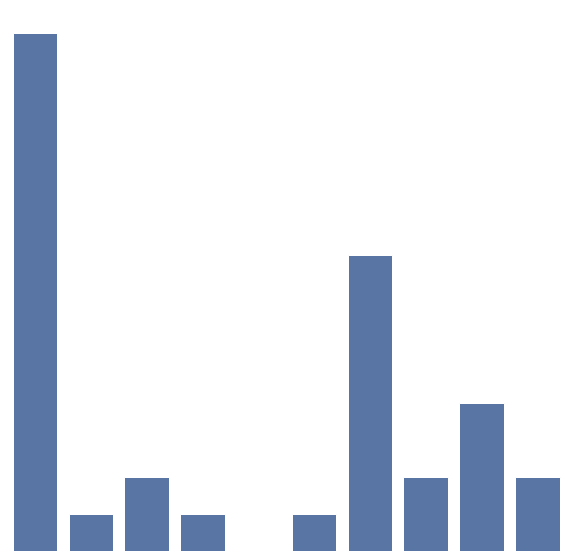
\includegraphics[width=0.49\textwidth]{images/aug/before.png}
\vrule
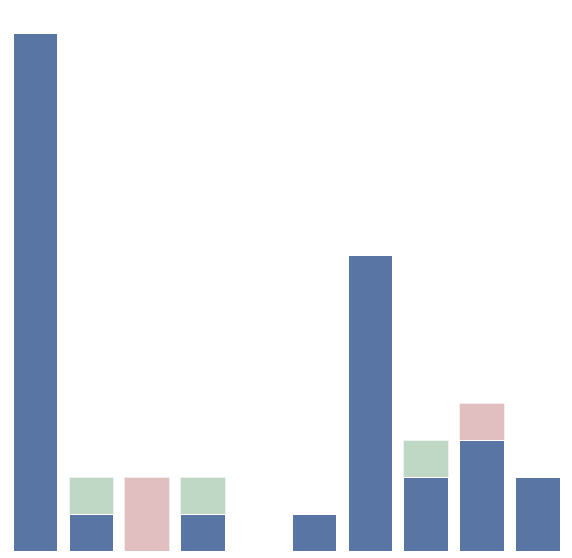
\includegraphics[width=0.49\textwidth]{images/aug/after.png}
\caption{Пример применения аугментация для длительностей графем для соседних символов. Слева - до, справа - после.}
\label{fig:aug}
\end{figure}

Опытным путем было выяснено, что аугментации помогают качеству звучания и уменьшают эффект переобучения (overfitting). Для тренировки генератора мэл-спектрограм мы применяли "биномиальную встряску" с $p=0.05$ для аугментации истинных длительностей.

Для тренировки генератора мэлов использовался тот же набор гиперпараметров, что и для предсказателя графем. Мы использование батч размера 64 для одной GPU в 16GB и увеличивали $\texttt{learning\_rate}$ пропорционально увеличению мощностей. Такая конфигурация позволила получить сходимость всего лишь за 200 эпох, что занимало около $8$ часа чистого времени на одной GPU и около $2$ часов на восьми GPU. Мы использовали обучение со смешанной точностью (mixed-precision,~\cite{micikevicius}), так как эмпирически было выявлено что такой подход позволяет получить почти двоекратное ускорение с сохранением качества.

Таким образом, процесс обучения обеих частей TalkNet'а на сервере DGX-1 может занимать всего порядка 2-ух часов. Это сравнимо меньше $2-3$ дней которые требуются модели Tacotron2~\cite{tacotron2}. Такая особенность связана прежде всего с эффектом неавторегрессионности, а также отсутствием операций основанных на механизмах внимания (attention), которые обычно занимают порядка $O(T^2)$ времени в зависимости от длины $T$.  % 3
\section{Результаты}

\subsection{Audio quality}

We conduct the MOS (mean opinion score) evaluation for generated speech using Amazon Mechanical Turk. We compared four types of samples: 1) ground truth speech, 2) ground truth mel-spectrogram converted to speech with WaveGlow, 3) Tacotron 2 + WaveGlow, and 4) TalkNet + WaveGlow. We used NVIDIA's implementation for Tacotron 2 and WaveGlow. We tested $100$ audio samples with $10$ people per sample. The scores ranged from $1.0$ to $5.0$ with a step of $0.5$. TalkNet speech quality comes quite close to Tacotron 2 (see Table~\ref{tab:mos}). 

\begin{table}[!ht]
\centering
\scalebox{1.0}{
\begin{tabular}{l c} 
\toprule
\textbf{Model} &
\textbf{MOS} \\
\midrule
Ground truth speech & $4.31 \pm 0.05$ \\
Ground truth mel + WaveGlow & $4.04 \pm 0.05$ \\
Tacotron 2 + WaveGlow & $3.85 \pm 0.06$ \\
% FastSpeech~\cite{Fastspeech2019} & $\star \pm \star$ \\
\midrule
TalkNet + WaveGlow & $3.74 \pm 0.07$ \\
\bottomrule
\end{tabular}
}
\caption{MOS scores with $95\%$ confidence interval}
\label{tab:mos}
\end{table}

TalkNet is very robust with respect to missing or repeated words compared to auto-regressive TTS models such as Tacotron 2 or Transformer TTS. We evaluated the robust\-ness of TalkNet on 50 hard sentences from FastSpeech paper~\cite{fastspeech} and found that TalkNet eliminates missed or repeated words.

\subsection{Inference latency}

In the inference mode, we first insert blank symbols into the tokenized input text between every two characters. The obtained sequence is passed through the grapheme duration predictor. The output of the grapheme duration predictor is then corrected for characters with $0$ duration. The corrected character sequence is expanded with each character repeated according to the predicted duration. The second network generates the mel-spectrogram from the expanded grapheme sequence.

We compare the TalkNet inference latency with Tacotron 2 and FastSpeech. We used an internal NVIDIA FastSpeech implementation since the original FastSpeech was not available at the moment of evaluation. To measure the latency, we generate mel-spectro\-grams with a batch size equal 1 for 2048  samples from LJSpeech dataset. The average mel-spectrogram length is $520$ frames. We benchmark the latency on one V100 GPU. TalkNet inference is significantly faster than Tacotron 2 and FastSpeech (see Table~\ref{tab:lats}). Since TalkNet  does not use an attention mechanism, the inference latency practically does not depend on the input length.

\begin{table}[!ht]
\centering
\scalebox{1.0}{
\begin{tabular}{l  l r} 
\toprule
\textbf{Model} & 
% \textbf{\thead{\# Batch\\size}} &
\textbf{\thead{Inference\\Latency, s}} &
\textbf{RTF} \\
\midrule
% Transformer TTS~\cite{TransformerTTS} & 1 & $6.735 \pm 3.969$ & $1.48 \pm 0.87$ \\
Tacotron 2~\cite{tacotron2}  &$0.817 \pm 1\cdot 10^{-2} $ & $7.56 \pm 0.01$ \\
FastSpeech~\cite{fastspeech}  & $0.029 \pm 2 \cdot {10}^{-4}$  & $221.01 \pm 1.75$ \\
\midrule
TalkNet  &  $0.019 \pm 1 \cdot {10}^{-5}$ & $328.65 \pm \ \ 4.76$ \\
%  & 4 &   $0.023 \pm 5 \cdot {10}^{-5}$ & $1048.80 \pm 21.75$ \\
%  & 8 &  $0.037 \pm 4 \cdot {10}^{-4}$ & $1340.09 \pm \ \ 8.90$ \\
\bottomrule
\end{tabular}
}
\caption{TalkNet inference latency for mel-spectrogram generation (without vocoder). The latency was measured with batch size $1$ using a V100 GPU and averaged over 2048 samples from LJSpeech. Latency and Real-Time-Factor (RTF) with $95\%$ confidence interval.}
\label{tab:lats}
\end{table}

\begin{figure}[!ht]
\centering
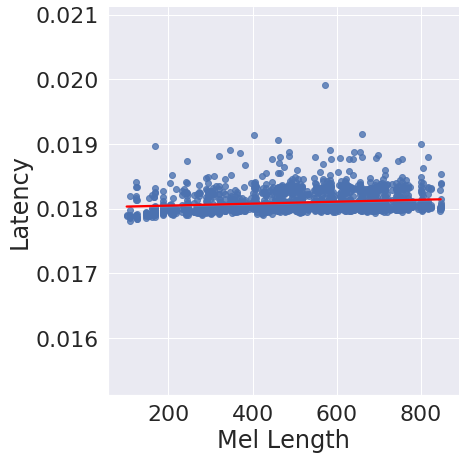
\includegraphics[width=1.0\textwidth]{images/len-lat.png}
\caption{Два шага TTS систем}
\label{fig:len-lat}
\end{figure}  % 4
\section*{Заключение}

В рамках данной работы был описан TalkNet~\cite{beliaev2020talknet}, нейронная система синтеза речи основанная по конволюционных сетях. Модель состоит из двух сверточных сетей: предиктора длительностей графем и генератора мэл-спектрограмм. Эта модель не требует другой предобученной системы в качестве учителя. Истинное выравнивание графем извлекается из выходных данных CTC для предварительно обученной модели распознавания речи.

Предсказывание длительностей явным образом практически исключает возможность пропущенных или повторяющихся слов. TalkNet достигает сопоставимого уровня качества речи с Tacotron 2 и FastSpeech. Данный подход также обладает свойством компактности. Он имеет только $10.8$ миллионов обучаемых параметров, что почти в 3 раза меньше, чем предлагают аналогичные нейронные модели: Tacotron 2 имеет $28.2$ миллионов, а FastSpeech имеет $30.1$ миллионов параметров. Обучение TalkNet занимает всего около $2$ часов на сервере с 8 графическими ускорителями V100. Параллельная генерация мэл-спектрограммы делает скорость обучения и вывода значительно быстрее конкурентов.

Современные генеративные модели все еще обладают рядом фундаментальных проблем, которые не позволяют считать задачу генерации речи решенной. Ценность этой работы заключается не только в предложенном и описанном подходе, позволяющем сильно сократить время и количество параметров, требуемых TTS системе, но и в трудностях, возникших при реализации, тестировании и сравнении подходов, указывающих на глобальные проблемы и очерчивающих границы применимости того или иного метода или модели.

В рамках данной работы можно выделить следующие основные результаты:
\begin{itemize}
    \item Проанализирована предметная область и существующие модели. Обозначены основные проблемы и намечены пути к их решению.
    \item Разработана новая неавторегрессионая конволюционная архитектура, не требующая предобученной TTS системы в качестве учителя.
    \item Произведены сравнение подходов и анализ результатов на качество и скорость. Предложенный подход показал сравнимое качество, являясь при этом быстрее и компактнее аналогичных методов.
\end{itemize}

Представленный подход, несмотря на свою простоту, открывает сразу несколько направлений для дальнейшего изучения и доработки.
\begin{itemize}
    \item Основное направление - улучшение качества. Следуя аналогичным статьям, переход с графем на звуковые фонемы должен помочь модели правильнее произносить звуки в словах.
    \item TalkNet multi-speaker. Многоголосовое расширение позволит проще искать данные для обучения и увеличит число потенциальных применений в индустрии.
\end{itemize}

Модель, скрипт для обучения и сгенерированные примеры будут выложены с открытым исходным кодом как часть библиотеки NeMo~\cite{nemo}. Автор благодарят Джона Коэна, Виталия Лаврухина, Джейсона Ли, Кристофера Паризьена и Жоао Фелипе Сантоса за полезные отзывы и рецензии.  % *

\bibliographystyle{ugost2008ls}
\bibliography{main.bib}

\end{document}
